\section{VLA-Adapter Methodology}\label{Section_methodology}

\subsection{Preliminary} \label{Subsection_preliminary}
We present the VLA-Adapter framework, as illustrated in Figure~\ref{Figure_framework}. This VLM follows the Prismatic-VLMs architecture \citep{Prismatic-2024}. It has $M$ layers. At timestep $t$, the input into VLM consists of $\{ \mathcal{X}_t^v, \mathcal{X}_t^g, \mathcal{L}_t, \mathcal{AQ}_t \}$: the 3rd-view image $\mathcal{X}_t^v$, the gripper image $\mathcal{X}_t^g$, the instruction $\mathcal{L}_t$, and additional ActionQuery $\mathcal{AQ}_t$. After inputting $\mathcal{X}_t^v$ and $\mathcal{X}_t^g$, the DINOv2 \citep{DINOv2-2024} and SigLIP \citep{SigLIP-2023} extract vision embeddings. $\mathcal{L}_t$ is tokenized. The outputs are the specified-layer Raw latent $\mathcal{{\cal C}}_t^\mathcal{R}$ and ActionQuery latent $\mathcal{{\cal C}}_t^\mathcal{AQ}$. They serve as the conditions for Policy.

\begin{figure}[!htbp]
	\centering
	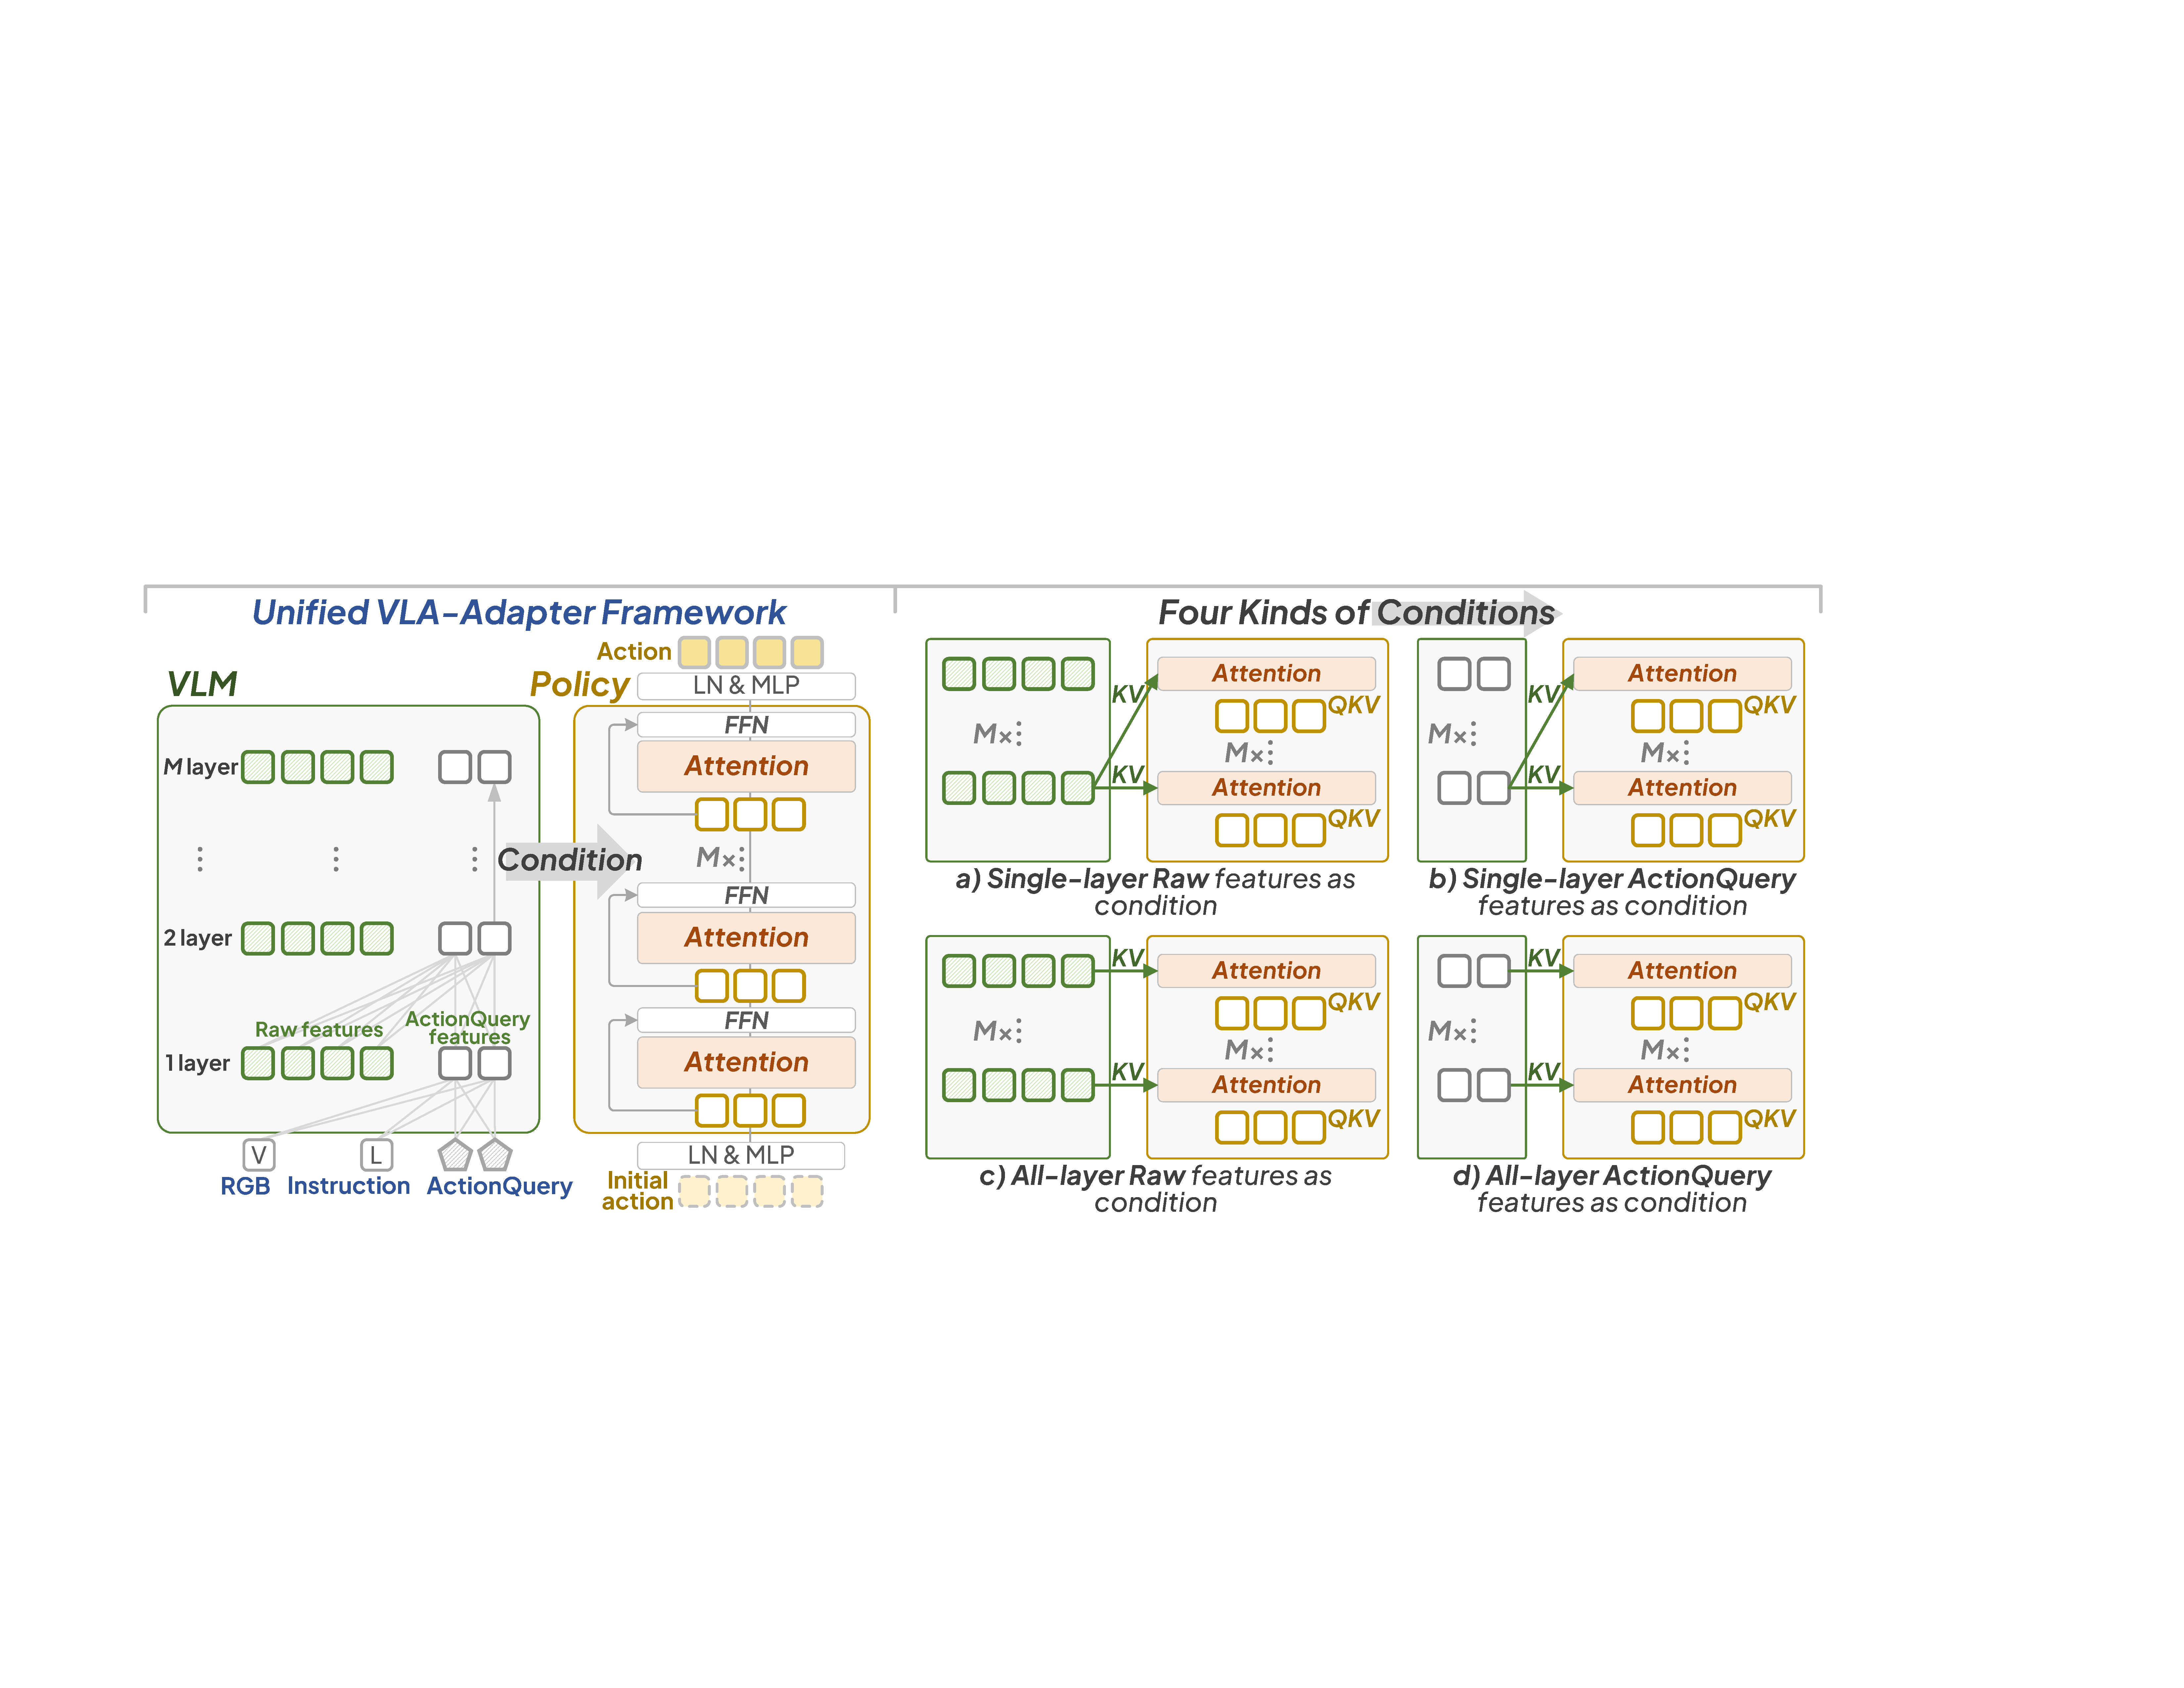
\includegraphics[width=0.97\textwidth]{Figures/Model.pdf}	
	\caption{The proposed VLA framework. The key components are the effective condition exploration and Attention design. ``\textit{Attention}" specifically includes cross attention with conditions and self attention with itself. In the ``\textit{Unified VLA-Adapter Framework}", ``\textit{Attention}" is the Bridge Attention as shown in Section \ref{Subsection_bridge_attention}. Four conditions about ``layer" and ``type" are given on the right.}\label{Figure_framework}
\end{figure}

\paragraph{Backbone.} To build a solid basis for research, we perform experiments of VLA-Adapter on different-scale backbones. The backbones select the Prismatic VLM trained on Qwen2.5-0.5B \citep{Qwen2-2024}, the Prismatic VLM trained on LLaMA2-7B \citep{LLaMA2-2023}, and OpenVLA-7B \citep{OpenVLA-2024} pre-trained on robotic data. The benefit gained from increasing backbone scale is limited in VLA-Adapter. The results are shown in Table \ref{Table_effectiveness} of Section \ref{sec41}. Therefore, to ensure efficiency, Qwen2.5-0.5B is our default backbone unless otherwise specified.

\subsection{Which Condition Is Essential for Bridging from VL to A?}\label{Subsection_condition}
Although existing methods have adopted various bridging paradigms from VL to A, their relative effectiveness remains inconclusive. This is mainly due to the differences in the design of the VLM and the Policy. To address this gap, we explore which type of perception information is essential for action generation in the Policy network. In summary, we mainly focus on the following questions:

\begin{description}
	\item[] \thinspace \textit{\textbf{Question 1.1.} Which layer of features within the VLM is more effective for the Policy network? }
	\item[] \thinspace \textit{\textbf{Question 1.2.} Are the ActionQuery features a better choice than the Raw features?}
\end{description}

To ensure compatibility with existing experimental protocols for representative work (e.g., $\pi_{0}$ \citep{pi0-2025}), we let the number of Policy layers be equal to that of VLM. At each layer of Policy, the action latent undergoes cross-attention with conditions and self-attention with itself. This iterative process ultimately yields the action output. Details of the Policy can be seen in Section \ref{Subsection_bridge_attention}.

\paragraph{Experimental Setting.} 

\begin{wrapfigure}{r}{8.8cm}
	\centering
	\vspace{-0.45cm}
	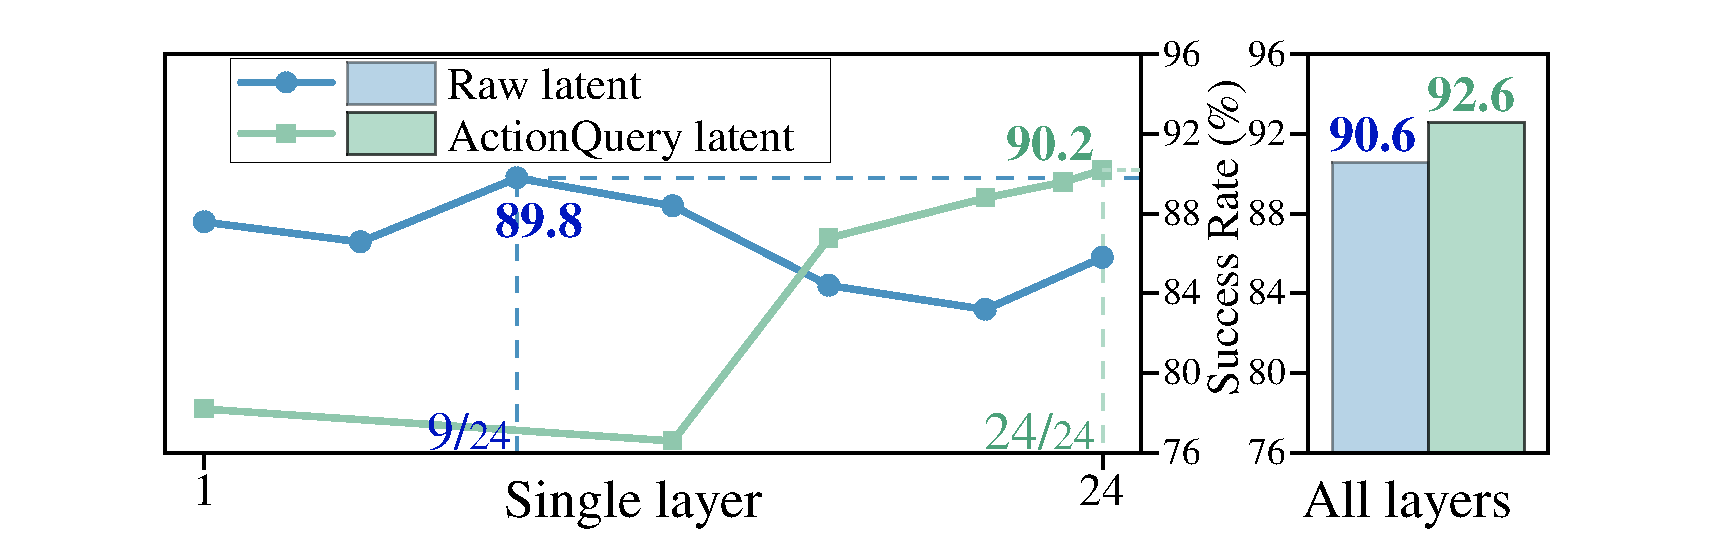
\includegraphics[width=0.6\textwidth]{Figures/Ablation_v1.pdf}
	\vspace{-0.25cm}
	\caption{Comparison of four conditions in the VLA-Adapter framework on the LIBERO-Long. Blue and Green lines are single-layer $\mathcal{{\cal C}}_t^\mathcal{R}$ and single-layer $\mathcal{{\cal C}}_t^\mathcal{AQ}$, as in Figure \ref{Figure_framework}a) and \ref{Figure_framework}b). Blue and Green columns are all-layer $\mathcal{{\cal C}}_t^\mathcal{R}$ and all-layer $\mathcal{{\cal C}}_t^\mathcal{AQ}$, as in Figure \ref{Figure_framework}c) and \ref{Figure_framework}d). The detailed results are shown in Appendix \ref{AppendixC}. Please note: the number of ActionQuery is 64 here. Its number is variable, similar to MetaQueries \citep{Metaquery-2025} in MLLM research; we will explore it in Section \ref{sec45}.}\label{Figure_condition}
	\vspace{-0.2cm}
\end{wrapfigure}

We evaluate four conditions in our framework. For \textit{\textbf{Question 1.1}}, to evaluate the effectiveness of the individual-layer information, we employ the single-layer latent as the conditions for the all-layer Policy, as shown in Figure \ref{Figure_framework}a) and \ref{Figure_framework}c). To evaluate the effectiveness of all-layer information, we feed each-layer latent into the corresponding-layer Policy, as shown in Figure \ref{Figure_framework}b) and \ref{Figure_framework}d). For \textit{\textbf{Question 1.2}}, to compare the effectiveness of the feature types, we use the $\mathcal{{\cal C}}_t^\mathcal{R}$ or $\mathcal{{\cal C}}_t^\mathcal{AQ}$ as conditions. The comparison on the LIBERO-Long \citep{LIBERO-2023}, which is the long-horizon and complex benchmark, the results are as shown in Figure \ref{Figure_condition}. We give the following key findings.


\begin{description}
	\item[] \thinspace \textit{\textbf{Key Finding 1.} Regarding $\mathcal{{\cal C}}_t^\mathcal{R}$, the middle-layer latent performs better than the deep-layer latent.} Deep-layer $\mathcal{{\cal C}}_t^\mathcal{R}$ is biased towards semantic information and less effective in action generation. The middle-layer $\mathcal{{\cal C}}_t^\mathcal{R}$ effectively integrates image and text information, retains richer multimodal details, and facilitates action generation.
\end{description}

\begin{description}
	\item[] \thinspace \textit{\textbf{Key Finding 2.} Regarding $\mathcal{{\cal C}}_t^\mathcal{AQ}$, deep-layer latent performs better than other-layer latent.} Since ActionQuery is trained from scratch, and deep-layer $\mathcal{{\cal C}}_t^\mathcal{AQ}$ aggregates richer multimodal details and is more effectively promoting action generation than the shallow layers.
\end{description}

\begin{description}
	\item[] \thinspace \textit{\textbf{Key Finding 3.} Multi-layer features perform better.} We observed that using all-layer features generally outperforms a single layer. Not only does it improve performance, but it also saves time on best layer selection during design. This design can be more universal.
\end{description}

\paragraph{Condition Determination.} Does VLA-Adapter rely exclusively $\mathcal{{\cal C}}_t^\mathcal{AQ}$ as conditions? The answer is no. While all-layer $\mathcal{{\cal C}}_t^\mathcal{AQ}$ outperforms $\mathcal{{\cal C}}_t^\mathcal{R}$, middle-layer $\mathcal{{\cal C}}_t^\mathcal{R}$ excels in some hard tasks. Comparison is shown in Table \ref{Table_condition_deter}. So, we aim to enhance performance by using certain knowledge from $\mathcal{{\cal C}}_t^\mathcal{R}$.

\begin{table}[!htbp]
	\centering
    \small
	\caption{Comparison of the $i$th-layer $\mathcal{{\cal C}}_t^\mathcal{R}$ and $\mathcal{{\cal C}}_t^\mathcal{AQ}$ in subtasks of LIBERO-Long.}\label{Table_condition_deter}%
	\begin{tabular}{c|cc|c|ccccccc}
		\toprule[1pt]
		$\mathcal{{\cal C}}_t^\mathcal{R}$ & 9     & 13   &$\mathcal{{\cal C}}_t^\mathcal{AQ}$& 1 & 13    & 17    & 21    & 23    & 24    & All \\
		\midrule[0.5pt]
		Subtask 7& \multicolumn{1}{c}{\textbf{90}} & \multicolumn{1}{c|}{82} & Subtask 7& 76    & 66    & 74    & 70    & 70    & 74    & 76 \\ 
		Subtask 9 &74&\textbf{84}&Subtask 9&78&62&58&72&72&84&78\\
		\bottomrule[1pt]
	\end{tabular}
\end{table}


\subsection{Policy with Bridge Attention}\label{Subsection_bridge_attention}

\paragraph{Overall.} For the simplicity of the model, we designed an L1-based Policy network. At $t$-th timestep, the input to Policy includes: $\{ \mathcal{{\cal C}}_t^\mathcal{R}, \mathcal{{\cal C}}_t^\mathcal{AQ}, {\bf A}^{\tau=0}_t , \mathcal{P}_t\} $. 
$\tau$ is the layer of Policy, and it has $\tau\in \mathbb{Z}^+$, $0 \leq \tau \leq M-1$. 
${\bf A}^{0}_t$ is the $H$-step initial action of all zeros, it is processed by LayerNorm (LN) and Multi Layer Perceptron (MLP) to obtain $\widetilde{\bf A}^0_t = \left[\widetilde{\bf a}^0_t, \widetilde{\bf a}^0_{t+1}, \dots, \widetilde{\bf a}^0_{t+H-1} \right]$. $\mathcal{P}_t$ is the proprioceptive state, and it is mapped through a two-layer MLP to obtain the proprio embedding ${\sigma _0}({\mathcal{P}_t})$. The output is the $H$-step action chunk ${\bf A}^{M-1}_t$. Each layer is composed of a Bridge Attention module and a Feed-Forward Network (FFN). The Bridge Attention architecture is shown in Figure \ref{Figure_bridge_attention}.

\begin{figure}[!htbp]
	\centering
	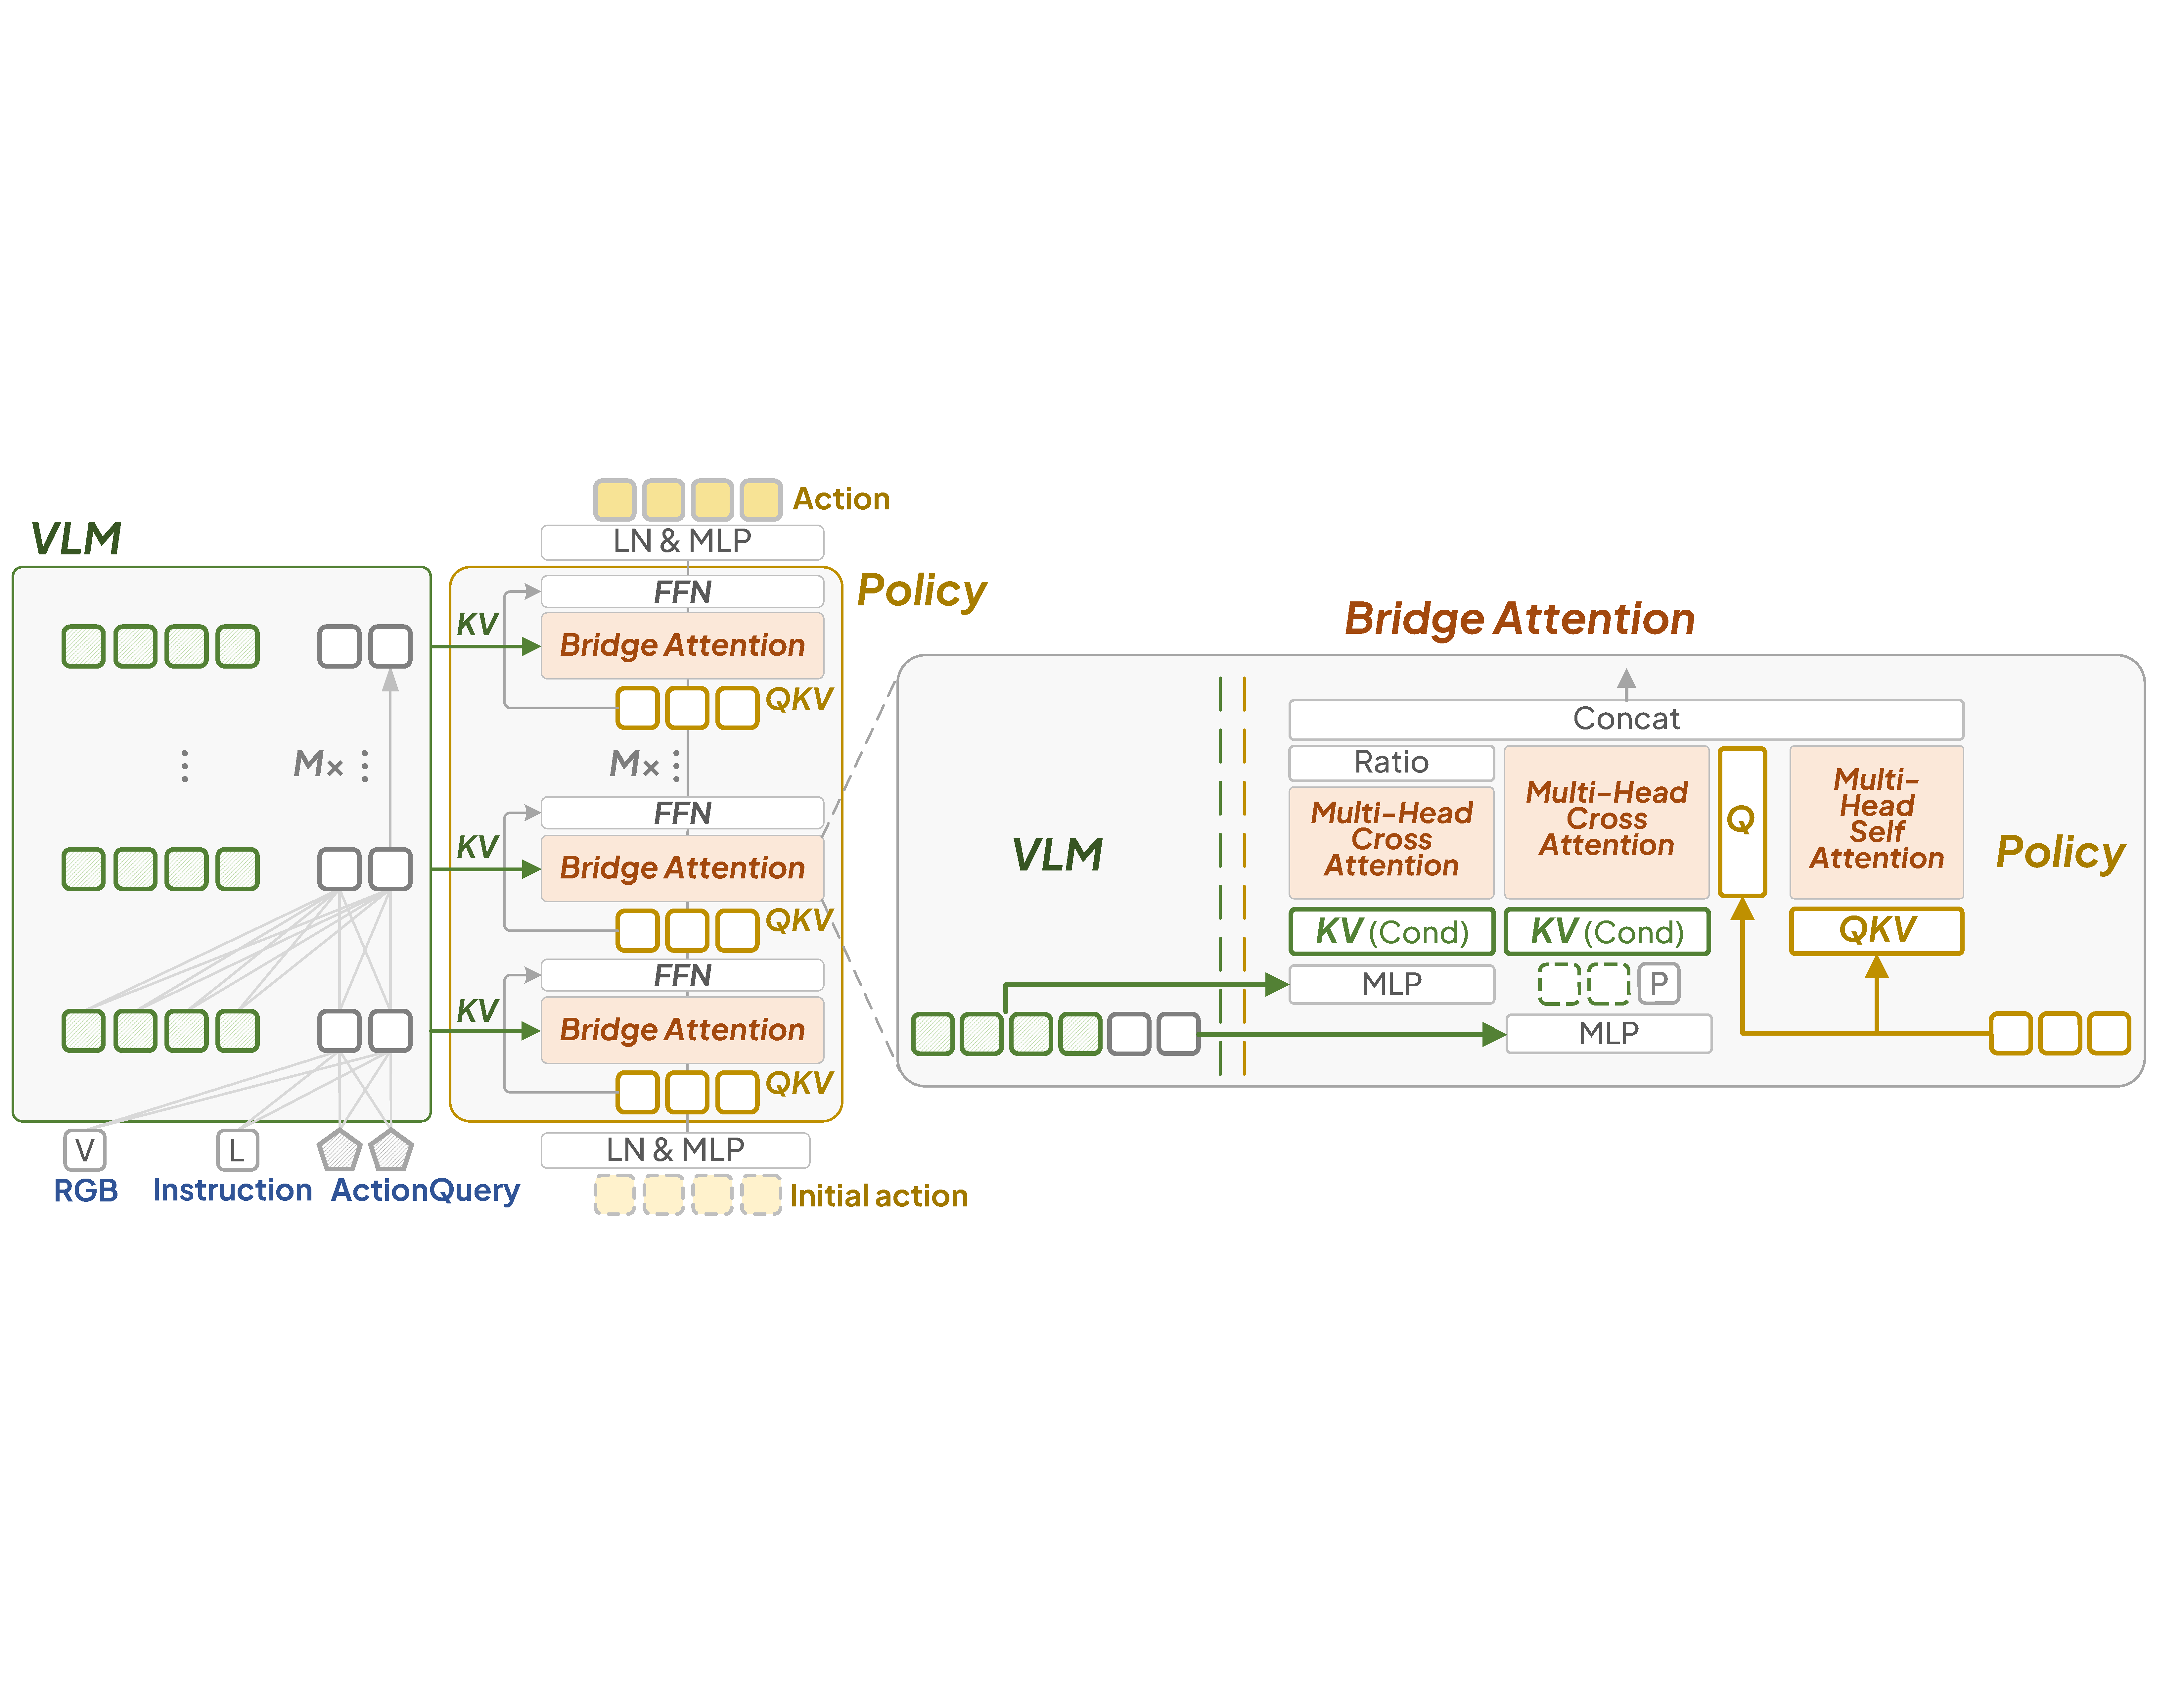
\includegraphics[width=0.97\textwidth]{Figures/Framework.pdf}	
	\caption{The Policy with Bridge Attention. The Policy parameters are only 97M when the backbone is Qwen2.5-0.5B. Each-layer $\mathcal{{\cal C}}_t^\mathcal{R}$ and $\mathcal{{\cal C}}_t^\mathcal{AQ}$ are integrated in Bridge Attention with the corresponding-layer action latent. Bridge Attention maps VL to Action to the greatest extent. The degree of $\mathcal{{\cal C}}_t^\mathcal{R}$ injection is learnable, ensuring the performance and stability of training.}\label{Figure_bridge_attention}
\end{figure} % 

\paragraph{Bridge Attention.}\label{sec331} 
The proposed Bridge Attention hopes to guide action generation to the greatest extent possible through the conditions $\mathcal{{\cal C}}_t^\mathcal{R}$ and $\mathcal{{\cal C}}_t^\mathcal{AQ}$. Each Bridge Attention consists of two cross attentions and one self attention. In the first cross attention, $\mathcal{{\cal C}}_t^\mathcal{R}$ is processed through an MLP $\sigma_1$ to obtain $K_1,V_1$. The action latent $\widetilde{\bf{A}}^\tau_t$ is used as the $Q_1$, and perform attention to get $\text{CA}_1\left(\widetilde{\bf{A}}^\tau_t,\sigma_1(\mathcal{{\cal C}}_t^\mathcal{R})\right)$. In the second cross attention, $\mathcal{{\cal C}}_t^\mathcal{AQ}$ needs to be concatenated with the ${\sigma _0}({\mathcal{P}_t})$ and passed through an MLP $\sigma_2$ to obtain $K_2,V_2$. $\widetilde{\bf{A}}^\tau_t$ is used as the $Q_2$ to get $\text{CA}_2\left(\widetilde{\bf{A}}^\tau_t,\sigma_2\left[\mathcal{{\cal C}}_t^\mathcal{AQ},{\sigma _0}({\mathcal{P}_t})\right]\right)$. In the self attention, $\widetilde{\bf{A}}^\tau_t$ is as $Q,K,V$, and there is $\text{SA}(\widetilde{\bf{A}}^\tau_t,\widetilde{\bf{A}}^\tau_t)$.

To selectively inject certain $\mathcal{{\cal C}}_t^\mathcal{R}$ into the action space of the Policy, we introduce a learning parameter Ratio $g$ to modulate the influence of $\text{CA}_1\left(\widetilde{\bf{A}}^\tau_t,\sigma_1(\mathcal{{\cal C}}_t^\mathcal{R})\right)$. $g$ is initialized to 0 value, and the $\tanh$ activation function is utilized $\tanh(g)\in[-1,1]$ to prevent extreme values from destabilizing the distribution \citep{LLaMA-Adapter-2024}. And then, the three attentions are concatenated to obtain $\widehat{\bf{A}}_t^\tau$:

\begin{equation}
\widehat{\bf{A}}_t^\tau = 
[\text{CA}_1\left(\widetilde{\bf{A}}^\tau_t,\sigma_1(\mathcal{C}_t^\mathcal{R})\right)\cdot \tanh(g), \text{CA}_2(\widetilde{\bf{A}}^\tau_t,\sigma_2[\mathcal{C}_t^\mathcal{AQ},  \sigma_0({\mathcal{P}_t})]), \text{SA}\left(\widetilde{\bf{A}}^\tau_t, \widetilde{\bf{A}}^\tau_t\right)].
\end{equation}

After Bridge Attention, $\widehat{\bf{A}}_t^\tau$ passes through a residual FFN to obtain $\widetilde{\bf A}^{\tau+1}_t$. Repeating the above process, we finally obtain $\widetilde{\bf A}^{M-1}_t$. The action chunk ${\bf A}^{M-1}_t$ is yielded by an LN and MLP layer. 

Additionally, we also design a DiT-based (Diffusion Transformer \citep{DiT-2023}) Policy. Since the diversity of Policy is not the focus of this paper, we put its details and the brief results in Appendix \ref{Appendix_DiT}. The results show that L1-based performance and inference speed are generally superior to those of the DiT-based approach. Therefore, VLA-Adapter chose the L1 architecture as the Policy.


\subsection{Training}\label{Subection_training}
The training is conducted end-to-end, with the Policy trained from scratch. Given a ground truth action trajectory ${{\bf{A}}_t}$ and action latent ${\bf{A}}_t^{\tau}$. We train VLA-Adapter model $\pi_\theta ( \cdot )$ with the objective:

\begin{equation}
\min_\theta \mathcal{J}(\theta) = \mathbb{E}_{\mathbf{A}_t, \mathcal{C}_t^{\mathcal{R}}, \mathcal{C}_t^{\mathcal{AQ}}, {\sigma _0}({\mathcal{P}_t}),\tau} \Big[\big\| \pi_\theta(\mathbf{A}_t^\tau, \mathcal{C}_t^{\mathcal{R}}, \mathcal{C}_t^{\mathcal{AQ}},{\sigma _0}({\mathcal{P}_t}),\tau) - \mathbf{A}_t \big\|_1\Big].
\end{equation}

For more details of training, please see Appendix \ref{AppendixE1}. 